\chapter{Introduction}
\label{chap:introduction}

{ \Large \leftwatermark{
\put(-76.5,-75){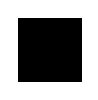
\includegraphics[scale=0.8]{img/thumbindex.eps}}  \put(-67,-66.5){ {\color{white} 1 }}
\put(-67,-91.5){ 2 }
\put(-67,-116.5){ 3 }
\put(-67,-141.5){ 4 }
\put(-67,-166.5){ 5 }
\put(-67,-191.5){ 6 }
\put(-67,-216.5){ 7 }
\put(-67,-241.5){ 8 }
\put(-67,-266.5){ 9 }
\put(-67,-291.5){ 10 }
\put(-67,-316.5){ 11 }
} \rightwatermark{
\put(346.5,-75){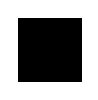
\includegraphics[scale=0.8]{img/thumbindex.eps}}  \put(350.5,-66.5){ {\color{white} 1 }}
\put(350.5,-91.5){ 2 }
\put(350.5,-116.5){ 3 }
\put(350.5,-141.5){ 4 }
\put(350.5,-166.5){ 5 }
\put(350.5,-191.5){ 6 }
\put(350.5,-216.5){ 7 }
\put(350.5,-241.5){ 8 }
\put(350.5,-266.5){ 9 }
\put(350.5,-291.5){ 10 }
\put(350.5,-316.5){ 11 }
}}

\newpage

\section{A short history on chromosomes and DNA} \label{intro_history}
In 1865 the Augustinian friar and scientist Gregor Mendel was the first to give a systematic account of the heredity of traits following specific laws \cite{Mendel_1866}. 
In the following decades it was discovered that during cell division a substance in the cell nucleus, dubbed \textsl{chromatin} (stainable substance) by German biologist Walther Flemming, was divided over the two halves of the cells during a process that Flemming called \textsl{mitosen}, or mitosis \cite{Schneider_1873,Flemming_1882,Cremer_2006}. 
A few years later, in 1890, German histologist Richard Altmann noted the presence of granules in cells that he believed were elementary organisms enclosed within cells, features later renamed ‘mitochondria’ by German microbiologist Carl Benda \cite{Altmann_1894,Benda_1898}. 
In 1888, German anatomist Wilhelm Waldeyer was the first to use the term \textsl{chromosomen} – chromosomes, meaning colored bodies – to describe the individual pieces of chromatin thread \cite{Waldeyer_1888,Cremer_2006}. 
In the last decade of the 19th century, the German biologist August Weismann proposed that the chromosomes were the bearers of hereditary material, which he called \textsl{keimplasma}, or germ plasm \cite{Weismann_1892}. 
At the time he was unaware of Mendel’s work. However, after its rediscovery at the turn of the century, the cytologists Walter Sutton, from the United States of America, and Theodor Boveri, from Germany, both showed that chromosomes follow Mendelian laws \cite{Sutton_1902,Boveri_1904,Boveri_1909,Crow_2002}. 

The chromosome theory of heredity quickly became the leading theory in the field that became known as genetics, a term introduced by the English biologist William Bateson in 1905 \cite{Keynes_2008}. 
Around the same time, he and his colleagues observed coupling between different traits in pea plants \cite{Bateson_1906,Lobo_2008}, leading the British biologist Thomas Morgan, upon further \textsl{Drosophila} studies, to state that ‘we find “associations of factors” that are located near together in the chromosomes’ \cite{Morgan_1911}. 
This led to the theory of linkage a few years later \cite{Morgan_1915}. 
It was several more decades before the normal human chromosome number was correctly defined as 46 by Indonesian cytogeneticist Joe Hin Tjio in 1956 \cite{Tjio_1956}. 
After that it took only a few more years, until 1959, for French scientists Lejeune, Gauthier and Turpin to connect Down syndrome to the presence of a small extra chromosome \cite{Lejeune_1959}.
One year later, the Philadelphia-based researchers Hungerford and Nowell discovered a small abnormal chromosome present in people with human chronic myelogenous leukemia, demonstrating the use of cytogenic techniques in diagnosis of hematological diseases \cite{Nowell_1960}. 
This chromosome was later named the ‘Philadelphia chromosome’ and shown to be the product of translocation between chromosomes 9 and 22 \cite{Rowley_1973}.

In the meantime, based on work by British physicist Maurice Wilkins and chemist Rosalind Franklin, American biologist James Watson and British physicist Francis Crick created the double-helix DNA model containing the four nucleotides – Adenine, Cytosine, Guanine and Thymine – which are paired A=T and G$\equiv$C \cite{Watson_1953,Wilkins_1953,Franklin_1953}. 
Several years later Crick and his team inferred – without being able to sequence – the triplet DNA-protein translation code \cite{Crick_1961,Yanofsky_2007}. 
However, it was not until the following decade, when British Chemist Frederick Sanger invented DNA sequencing methods, that the DNA sequence itself could be read \cite{Sanger_1975,Sanger_1977}. 
In 1963, it was discovered that apart from the nucleus, mitochondria also contained DNA \cite{Nass_1963}. 
In 1983, Huntington’s disease was the first human disease to be linked to a specific genomic marker \cite{Gusella_1983}. 
In the following years more diseases were linked to genomic markers and genetic diagnostics expanded from analysis of chromosomes to inclusion of DNA analysis. 
After the invention of Polymerase Chain Reaction (PCR), DNA analysis became much easier \cite{Saiki_1985,Saiki_1988} and at the turn of the 21st century scientists were able to create a draft sequence of the human genome \cite{Lander_2001,Venter_2001}. 

The introduction of so-called next-generation sequencing in 2005 ushered in the start of yet another era \cite{Mardis_2013}. 
Sequencing costs decreased rapidly to the point that a whole genome can now be sequenced for less than 1000 dollars \cite{Goodwin_2016}, opening up new possibilities for human genome analysis and bringing the fields of cytogenetics and molecular genetics closer together\footnote{Paragraph 1.1 suggests a logical and continuous timeline between discoveries. However, many of those discoveries were heavily contested and others were made by several research groups independently around the same time. This means that the history told in this paragraph could just as well have contained other names. Their omission is not meant to discredit their scientific contribution, but this introduction is too short to give a more nuanced vision of the scientific progress in genetics.}. 



\section{Human genome variation} \label{intro_variation}
With improving genomic analysis techniques came increasing knowledge about the composition of the human genome. 
When comparing any two individuals, their six billion base pair human genome will show many differences, or DNA variants. On average, everyone has around three million DNA variants that differ from the major allele present in the population, of which 10.000-11.000 are non-synonymous variants that change the triplet code and result in an amino-acid change of a protein \cite{Durbin_2010}. 
Most of those variations do not cause disease but, as will be discussed in section 1.6, some variants are associated with or can contribute to a congenital disorder or a predisposition for the development of a disease. 

Several types of DNA variants can be distinguished. The smallest are Single Nucleotide Variants (SNVs) and indels: insertions or deletions of one or more bases (Figure \ref{fig:Introduction_Fig1}A-D). 
When a larger stretch of DNA is lost or duplicated, the variant is considered to be structural variation (SV) and the term Copy Number Variation (CNV) is used (Figure \ref{fig:Introduction_Fig1}E-H). 
The size threshold to distinguish a large indel from a small CNV is arbitrary, and different definitions are used in literature. While 1 kb was traditionally used as the lower threshold for CNVs, variants larger than 50 bp are now labelled as CNVs \cite{Redon_2006,Tan_2014,Wilfert_2017}. 
In formal notation, duplication is regarded as a tandem duplication, i.e. insertion of a duplicate sequence, following directly 3’of the original copy (figure \ref{fig:Introduction_Fig1}F), leaving the formal term ‘insertions’ to signify all other nucleotide insertions \cite{den_Dunnen_2016} (Figure \ref{fig:Introduction_Fig1}D and H). 
However, in practice, the term duplication is used in a broader sense for copy number gains that can also include translocational insertions \cite{Kang_2010,Hanemaaijer_2012}. 
One subset of duplications is repeat expansions in which a repeated nucleotide sequence is extended. 
An example of this is the CAG repeat that is extended in Huntington disease \cite{Rubinsztein_1996}. 
Another type of SV are translocations, in which terminal parts of chromosomes are exchanged (figure \ref{fig:Introduction_Fig1}I). 
In reciprocal translocations both derivative chromosomes are present without an apparent net loss or gain of chromosomal content, but in so-called unbalanced translocations, the translocation results in loss of part of one chromosome and gain of part of another chromosome \cite{Maithripala_2017}. 
In Robertsonian translocations, two acrocentric chromosomes are connected at the centromere \cite{Robertson_1916} (Figure \ref{fig:Introduction_Fig1}J). 
A further type of DNA variation are inversions in which a nucleotide sequence is replaced by its reverse complement sequence \cite{Sudmant_2015,den_Dunnen_2016} (Figure \ref{fig:Introduction_Fig1}K). 
While reciprocal translocations and inversions are balanced events in principle, deletions or insertions are often present around the breakpoints in both types of variations \cite{Sudmant_2015,Simioni_2017}. 
A further type of chromosomal variation are aneuploidies, in which whole chromosomes are lost or gained (and can be considered as whole chromosome CNVs), such as in Down syndrome (Figure \ref{fig:Introduction_Fig1}L).  


\begin{figure}[!ht]
	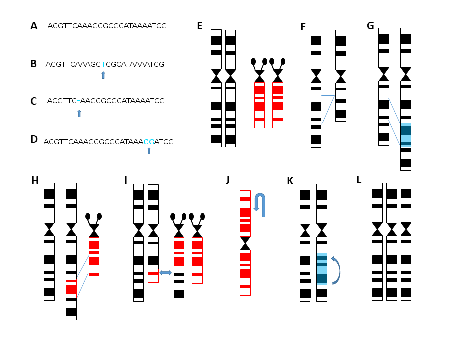
\includegraphics[width=1.0\linewidth]{img/Introduction_Fig1}
	\caption[Human genome variation types]{Human genome variation types: A) genomic base sequence, B) Single nucleotide variant, C) Indel: one base deletion, D) Indel: two base insertion, E) Two sets of chromosomes, F) CNV: Deletion, G) CNV: duplication, H) CNV: insertion, I) Reciprocal translocation, J) Robertsonian translocation, K) Inversion, L) Aneuploidy: trisomy}
	\label{fig:Introduction_Fig1}
\end{figure}



\section{Conventional techniques for variant detection} \label{intro_traditional}
Over the years many different techniques have been developed to detect and chart the DNA constitution. 
The earliest was karyotyping, the technique used by Tjio and Levan, in which metaphase spreads are made that enable analysis of chromosomes using a microscope \cite{Tjio_1956}. 
The development of chromosome staining techniques, such as Q,- C-, G- and R-banding, increased the resolution to a maximum of 5 Mb and enabled detection of smaller aberrations as well as more-specific determination of known variations \cite{Hamerton_1972,Liu_2015}. 
In situ hybridization techniques using radio- or fluorescent-labelled probes enabled detection of the presence and localization of specific parts of chromosomes \cite{Gall_1969,Bauman_1980,Levsky_2003}. 
It is particularly the latter, Fluorescence In Situ Hybridization (FISH), that paved the way for subchromosomal structural analysis, making it possible to detect microdeletions of several hundreds of kilobases (kb) \cite{Cui_2016}. 
Further developments of this technique, such as fiber-FISH, increased the resolution to 50 kb using mechanically stretched chromosomes \cite{Raap_1996}.
While these molecular techniques greatly advanced cytogenetics, analysis of solid tumors remained difficult because often no high-quality metaphases can be produced. 
Comparative Genomic Hybridization (CGH), an adaptation of FISH procedures, in which all patient DNA is fluorescently labelled and hybridized together with differently labelled reference DNA to high quality metaphases of a normal cell line enabled evaluation of aneuploidies, unbalanced translocations and CNVs \cite{Kallioniemi_1992}.
In other words, all types of variations resulting in loss or gain of chromosomal material could be detected genome-wide to a maximum resolution of 10 Mb for deletions and 2 Mb for amplifications, without the need of patient metaphase spreads \cite{James_1999b}. 
The same principle was used in array-CGH but, instead of metaphase spreads, a series of probes were used as the hybridization target, making it possible to detect CNVs smaller than 1 kb depending on the number and placing of the probes \cite{Pinkel_1998,Boone_2010}. 
Using knowledge gained by earlier sequencing projects, it became possible to target specific SNPs, enabling the array to be used not only for CNV detection, but also as a genotyping tool \cite{Wang_1998}. 
A targeted technique to further enhance the resolution for CNV detection is Multiplex-Ligation Probe Amplification (MLPA), in which several targeted stretches of DNA are amplified in one experiment, after which a relative comparison is done within a series of samples. 
Depending on the included targets, deletions or duplications of single exons can be detected \cite{Schouten_2002}.

Where cytogenetics and molecular cytogenetics focused on the detection of structural variations, including copy-neutral variations and aneuploidies (figure \ref{fig:Introduction_Fig1}E-L), molecular genetics focused on the detection of the nucleotide sequence, searching for SNVs, indels and repeat expansions (figure \ref{fig:Introduction_Fig1}A-D). 
Often, Sanger sequencing was the method of choice here. 
However, only a short stretch of DNA of a single sample can be analyzed in a single experiment using this technique. 

Variants are not always expected to be present in all cells from all tissues, as is the case with genetic mosaicism, including mitochondrial heteroplasmy, as well as in cancer. 
In karyotyping or FISH, a separate analysis is performed for each cell. 
By analyzing a large number of metaphases or nuclei, mosaicisms can be detected or excluded with high probability in the tissue studied \cite{Hook_1977,Sikkema_1997,Wolff_2007}. 
Several DNA-based methods are also able to assess the presence of low fractions of a certain type of DNA in a larger pool. 
Real-time quantitative PCR measures fluorescence after each PCR cycle, then, through comparison with samples having a known concentration, fractions of targeted DNA stretches can be calculated for a sample \cite{Heid_1996}. 
Quantitative fluorescent (QF-)PCR measures the DNA concentration after a fixed number of PCR cycles \cite{Eggeling_1993}. 
A more recent addition is digital droplet PCR (ddPCR), where DNA fragments are encapsulated in oil droplets. 
For each droplet it is determined if a specific DNA sequence is present or not. Because tens of thousands droplets can be assessed in a single experiment, this technique has a high sensitivity for low-abundance variations \cite{Hindson_2011}.

It is no coincidence that so many techniques have been developed for DNA analysis, as each technique has distinct strengths and weaknesses. 
In karyotyping at low resolution, chromosome specific analysis can be done for the whole genome of a single cell. 
FISH increases resolution, but only gives information about targeted regions, while array gives high resolution whole genome information, but can’t distinguish alleles and thus misses copy neutral structural variations. 
MLPA and Sanger sequencing have even higher resolution – the latter up to a single base pair – but, in a single experiment, are limited to analysis of a small part of the genome. 
Therefore, using these conventional techniques to find all types of variations present in a single sample requires many different experiments. 


\section[Next-generation sequencing]{Next-generation sequencing}\label{intro_ngs}
In the mid-2000s, massive parallel sequencing was developed. With the introduction of this method, there was an immediate 50,000 fold drop in sequencing costs, resulting in the label ‘next-generation sequencing’ (NGS) \cite{Goodwin_2016}. 
NGS can be used for DNA as well as RNA sequencing. 
While the term NGS might suggest a single technique, it is in fact an umbrella-term encompassing many different technologies that sequence many DNA or RNA fragments in parallel and infer a read of the nucleotide sequence of each fragment.
The first NGS platform available was developed by 454 Life Sciences using a pyrosequencing strategy \cite{Margulies_2005}. 
Solexa then introduced NGS using reversible dye terminator chemistry \cite{Bentley_2008} and Ion Torrent a non-optical system based on pH changes on nucleotide incorporation \cite{Rothberg_2011}. 
With these technologies being acquired by Roche, Illumina and Life Technologies, three strong contenders entered the short-read sequencing market. Other platforms focus on sequencing long single DNA molecules, such as Pacific Biosystems \cite{Eid_2009} and Oxford NanoPore \cite{Clarke_2009}, making use of real-time measurements of fluorescent signals and changes in current, respectively. 
Other contenders have since entered and left the NGS market, all using different chemistry and measurement tools. Because of this, technical bias is different from one technique to the other, although some genomic regions still remain a challenge for all platforms. 

Although the exact methods used differ between different NGS techniques, their general approach is similar, as shown in figure \ref{fig:Introduction_Fig2}, although the strong and weak points vary between the platforms. 
For NGS DNA analysis, various input materials can be used. 
Some contain fragmented DNA, such as blood plasma or formalin-fixed paraffin-embedded (FFPE) material (figure \ref{fig:Introduction_Fig2}A), while others contain high quality DNA, for example white blood cells, bone marrow or cultured cells (figure \ref{fig:Introduction_Fig2}B). 
The first step in all DNA NGS procedures is to isolate DNA from the material. 
In the materials where the DNA is already fragmented, short DNA fragments are isolated (figure \ref{fig:Introduction_Fig2}C).

\begin{figure}
	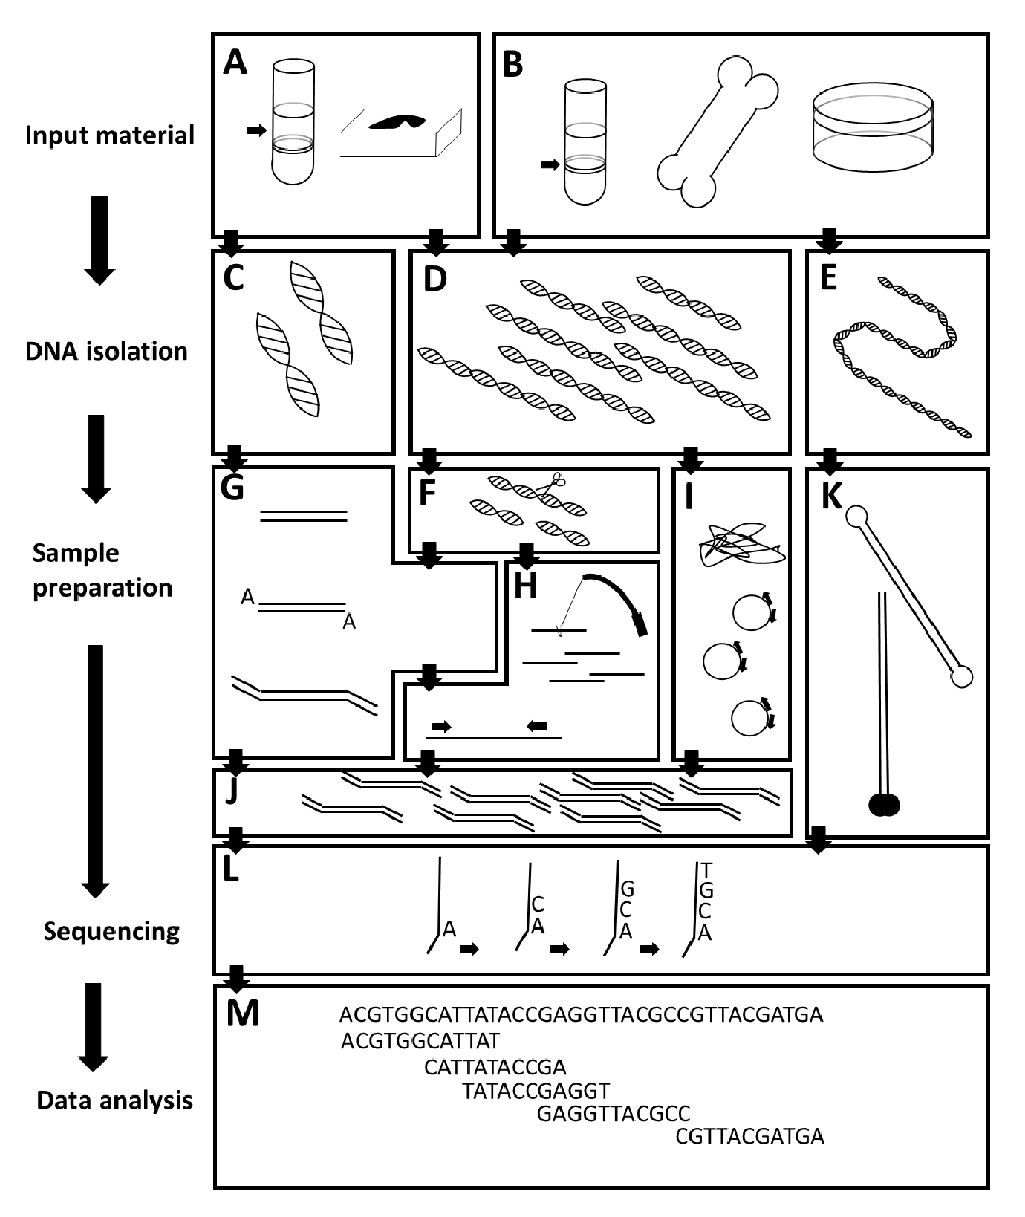
\includegraphics[width=1.0\linewidth]{img/Introduction_Fig2}
	\caption[DNA Next-generation sequencing workflows]{DNA Next-generation sequencing workflows. A) Sources of fragmented DNA, such as blood plasma or FFPE material, B) sources of high quality DNA, such as white blood cells, bone marrow cells or cultured cells, C) isolated fragmented DNA, D) isolated high-quality DNA, E) isolated long fragments of DNA, F) DNA fragmentation, G) sample preparation (end-repair, dA-tailing and adapter ligation), H) enrichment via capturing or amplicon sequencing), I) alternative sample preparation, such as Targeted Locus Amplification or ATAC-seq, J) PCR, K) long-read sequencing sample preparation, L) sequencing of the DNA, M) data analysis to transform sequenced DNA into sequence reads and subsequently into sample-specific genomic sequences.}
	\label{fig:Introduction_Fig2}
\end{figure}

Source materials containing higher quality DNA can give rise to longer DNA-fragments (figure \ref{fig:Introduction_Fig2}D) or even very long DNA fragments, if DNA breakage is prevented during isolation (figure \ref{fig:Introduction_Fig2}E). 
The short-read sequencing methods work best when using relatively short DNA fragments. 
For these techniques, DNA needs to be fragmented if the input fragments are too long (figure \ref{fig:Introduction_Fig2}F). 
The most basic short-read strategy is whole genome sequencing (WGS). 
Sample preparation consists of adding so-called ‘adapters’ to DNA-fragments, thus making the fragments suitable for sequencing (figure \ref{fig:Introduction_Fig2}G). 
If only a part of the genome needs to be sequenced, the DNA can be enriched for the sequences of interest (figure \ref{fig:Introduction_Fig2}H). 
Various methods can be used to reach this goal, such as DNA capturing, in which short RNA or DNA sequences complementary to the region of interest called ‘baits’ are used to fish out specific parts of the genome.
A second method is amplicon sequencing. Here, similar to Sanger sequencing, two primers are used that bind to their complementary sequence and copy the genomic sequence in between the primers. Such enrichment techniques are used in, for instance, whole exome sequencing (WES) and gene panels that target specific genes of interest. 
In addition to these ‘standard’ sample preparation methods, alternative sample preparations can be performed that have a different perspective on the genome (figure \ref{fig:Introduction_Fig2}I), for instance using proximity ligation \cite{Spielmann_2018}, targeted locus amplification \cite{de_Vree_2014}, or chromatin-immunoprecipitation or by enzymatic digestion \cite{Jiang_2018}.
 
The final step in the sample preparation is PCR amplification to produce sufficient fragments of the DNA of interest to be sequenced (figure \ref{fig:Introduction_Fig2}J). 
Alternatively, long-read sample preparation methods can be used (figure \ref{fig:Introduction_Fig2}K). 
The bases of the DNA fragments are subsequently read by the sequencer (figure \ref{fig:Introduction_Fig2}L). 
Data analysis is then carried to determine the nucleotide sequence of the DNA fragments, and the genomic sequence of the sample can be inferred through further processing, for instance through alignment of sequenced reads to a reference genome (figure \ref{fig:Introduction_Fig2}M). 
Once the genomic sequence is inferred as far as possible, the presence or absence of variants can be de determined and interpreted in the context of a scientific or diagnostic question. 
An important step in variant calling and interpretation is to distinguish true positive and negative results from false ones. 
Knowing where variants can be missed, or where artefacts are more likely to occur, can be important for making a correct interpretation. 
Moreover, if the cause of artefacts is known, analysis procedures can be adapted to counteract sources of bias and create a more optimal balance between sensitivity and specificity. 


\section[Technical bias and error rates]{Technical bias and error rates}\label{intro_bias}
Where conventional techniques have proven their worth in genetic diagnostics, NGS procedures and analysis still need to be optimized, and refining the methods to improve their sensitivity and specificity remains a challenge. 
The aim of the different NGS techniques is to measure the exact nucleotide sequences of the DNA fragments. 
However, technical bias and sequencing errors create noise, resulting in some of the nucleotides in a sequence read being called incorrectly. 
This error rate is much higher for long-read technologies than for short-read sequencing. Depending on the chemistry and platform used, error rates range from 0.1\% to 15\% \cite{Goodwin_2016}. 
These error rates are presented as base quality scores and, when several reads are combined to infer a genotype, as a genotype quality score \cite{Nielsen_2011}. 
However, it has been shown that discordance rates between short-read samples that have been analyzed twice are higher than would be expected using the genotype quality scores \cite{Wall_2014,Schirmer_2015}, which suggests that error rates are higher than the sequence data lead us to believe. 
Whereas some of the sequencing errors are random, each type of sequencer, as well as each experimental design, has its own systematic biases that occur at specific sequence patterns, inverted repeats or homopolymers \cite{Nakamura_2011,Schirmer_2015}. 
Because some of the errors are made during PCR amplification, base quality scores are not always sufficient to determine the chance that a specific base is called correctly for a sequenced DNA fragment.
This is especially important when the aberration of interest is expected to occur in only a subset of the analyzed DNA fragments, as is the case for germline and somatic mosaic variants and for non-invasive prenatal testing (NIPT), where fetal DNA is analyzed in the presence of maternal DNA, because fewer sequence reads will be present to support a genotype call. 
An important contributor to the creation of bias during PCR is the GC percentage in the DNA fragment. If a high (\textgreater65\%) or low (\textless12\%) percentage of guanine or cytosine bases are present, the DNA fragments are barely amplified during PCR, with the amplification efficiency gradually increasing with GC percentages closer to 50\% \cite{Aird_2011}. 
With each PCR cycle needed in the experiment, the GC bias will grow, although this bias can also occur during PCR-steps that are part of the sequencing procedure itself \cite{Roeh_2017}. 
The severity of this bias can differ between samples and experiments. 
An extra effect of using many PCR cycles in sample preparation is that the number of reads originating from the same DNA fragment, called duplicate reads, will grow. 
This can lead to a risk of overestimating the effective coverage and sensitivity as well as the chance of amplifying errors occurring during extension in early PCR cycles, thus reducing specificity.  

For WGS, fewer PCR cycles are usually needed in the sample preparation, leading to a relatively even coverage between different genomic regions. 
However, targeted techniques such as WES and targeted NGS (tNGS) that rely on selective amplification of genomic regions of interest require PCR during sample preparation. 
In general, the rule applies that the lower the amount of input material or the smaller the targeted region, the more PCR cycles are needed, up to more than 30 cycles for some procedures. 
At 30 PCR cycles, over a billion copies of the same original DNA fragment are generated. 
In contrast, after 10 PCR cycles, just over one thousand copies are present. 
When randomly sheared DNA fragments are amplified and sequenced, duplicate reads can, to a certain extent, be identified based on the fact that they have an (almost) identical sequence. 
However, in amplicon-based sequencing, which uses primers to amplify a region of interest, it is expected that different original DNA fragments give rise to reads with the same sequence. 
This makes it more difficult to distinguish those reads from each other, unless separate molecular identifiers are used. 

But, even when all technical bias is corrected for, not all parts of the genome are accessible, especially in short-read sequencing. 
Many parts of the genome are not unique, for instance genes that have pseudogenes \cite{Mandelker_2016}. 
When a DNA-fragment originating from such a region is sequenced, there is no way to determine from the sequenced read itself if it is informative for the region of interest or for the other region that has the same sequence. 


\section{DNA variant detection in genome diagnostics} \label{intro_diagnostics}
In current genome diagnostics many of the DNA variant detection methods described in sections 1.3 and 1.4 are used. 
The types of variations that are searched for, as shown in figure 1.1, are different for different diagnostic questions. 
Moreover, the variants being examined can be present in only some of the cells – and therefore only part of the DNA analyzed – as discussed earlier. 
In the paragraphs below I discuss three important types of variants that need specific analysis and interpretation approaches: germline variants, somatic variants and variants found in prenatal testing. 

\subsection{Germline variants}
Germline variants are present at the formation of the zygote and, in principle, are present in all cells, including the germline \cite{Griffiths_2000}. 
For genetic analysis, white blood cells or fibroblasts provide a source of high-quality DNA. 
Germline variants can be transmitted from parent to child and can therefore result in multiple affected relatives within a family. 
Depending on the nature of the variants, a disease phenotype may develop during childhood, or adulthood, or even not at all. For Mendelian diseases the inheritance pattern for variants in autosomal chromosomes (i.e. chromosomes 1-22) can be autosomal dominant (AD) or autosomal recessive (AR). 
In AD inheritance, a variant in only one of the alleles can result in the disease phenotype. 
In AR inheritance, both parents transmit a pathogenic variant. 
Variants present in sex-chromosomes or mitochondria have different inheritance patterns. 
Because men carry one copy of each sex chromosome, a sex-chromosome-related recessive trait will result in a phenotype when a single copy of the causal variant is present. 
Mitochondria are always transmitted from mother to child, leading to phenotypes caused by mitochondrial variants only being inherited through the maternal line. 

One example of an AD hereditary disease is Lynch syndrome, one of the most common cancer predisposition syndromes. 
In Lynch syndrome, SNVs, indels, intragenic deletions or duplications cause a deficiency in the mismatch repair system that significantly increases the risk of developing cancer compared to the general population, although, as in other cancer-predisposing syndromes, not all carriers of pathogenic variants develop cancer \cite{Tutlewska_2013,Talseth_Palmer_2016}. 
It is estimated that around 1 in 300 people carry a pathogenic variant in one of the genes associated with Lynch syndrome \cite{Cancernet_2005}. 
One of the most common AR disorders is cystic fibrosis, which leads to dysfunctional chloride channels that cause thickened mucus and affects around 1 in 3500 individuals in Europe \cite{Yu_2018,Scotet_2012}. 
Children with cystic fibrosis often inherit a non-functional allele of the \textsl{CFTR} gene from both of their parents, who themselves don’t present with the disease phenotype because they have a functional copy of the gene. 
An example of a common recessive X-linked trait is red-green color-blindness, which affects 1 in 12 males and 1 in 200 females in populations with Northern-European ancestry \cite{Geneticshomereference_2019}. 
The prevalence of mitochondrial diseases is highly dependent on the population and is associated with, among other conditions, neurological diseases and ataxia \cite{Chinnery_2018}.

It is also possible that variants appear \textsl{de novo} during de formation of the gametes. 
\textsl{De novo} means that a variant is found in an individual even though neither of the parents carry this variant. 
Such a variant can arise through mistakes in copying DNA for SNVs and indels, through errors in crossing over for SVs, or through non-disjunction for aneuploidies. 
Examples of syndromes caused by SVs are Down syndrome (trisomy 21), Klinefelter syndrome (XXY), Turner syndrome (X0), Di-George syndrome (del 22q11) and the 1q21.1 microduplication syndrome.


\subsection {Somatic variants}
When a DNA variant is not present in the zygote but rather originates from a later cell division, it is called a somatic variant. 
If such a variant originates during embryonic development, it will be present in many cells; if it occurs later in life, it may be present in a small number of cells \cite{Frank_2014}. 
Some of the syndromes mentioned in the previous paragraph, Down syndrome and Turner syndrome for instance, can have their origin not only in germ cells, but also be the result of somatic mosaics. 
Mosaics may not lead to a clinical abnormal phenotype, depending on the distribution of the somatic variants over cells and tissues. 
Low level mosaics in parents that include their germ cells may be difficult to distinguish from \textsl{de novo} cases discussed in the previous section. 
Mosaics may also arise through a germline variation with a rescued cell-line in which the variation is eliminated \cite{Devlin_2004,Hook_2014}. 

Some disorders such as segmental neurofibromatosis \cite{Sobjanek_2014} or McCune-Albright syndrome \cite{Dumitrescu_2008}, in which parts of the body are affected while other parts are unaffected, are caused by mosaics. 
In cancer, somatic variants are the main cause of tumorigenesis. 
A tumor can develop when a gene variant causes uncontrolled cell division, as is the case with the Philadelphia chromosome \cite{Kang_2016}, or fails to lead the cell into appropriate cell-death, as is the case with variations affecting the \textsl{MYC} gene \cite{Dominguez_Sola_2014}. 
A cell that develops such a variant can then grow into a clonal population, which can later on develop into further subclones, together constituting the tumor cells \cite{Nowell_1976,Naugler_2010,McGranahan_2017}. 
In advanced disease stages, some variants can be present in a high percentage of cells. 
However, in earlier stages, after treatment or when a new variant has arisen in a subclone, it can be the case that only a small percentage of the cells analyzed carry the variant. 
In addition, tumor samples sent in for analysis typically contain both tumor cells and normal cells (e.g. lymphocytes or stromal cells), which adds to the mosaic nature of gene variants in these samples.

Somatic variants in tumor or hematological cells can consist of all the variant types described in section 1.2. 
However, while large structural variants, including aneuploidies, are rare events when looking at germline variants, they are more prevalent in cancer cells, where complex aberrant karyotypes are also seen. 
The main challenge for somatic variant detection in tumors is the possible presence of a wide variety of DNA variants and, sometimes balanced, chromosomal aberrations in a low percentage of the cells or DNA to be analyzed. 
In addition, the material containing the variations, such as bone marrow or tumor material, is harder to come by and often of lower quality than that used for germline variation detection.


\subsection{Prenatal testing}
Genetic variants can also be detected prenatally. 
Conventionally, such tests are offered to pregnant women at an elevated risk of carrying a child with a chromosomal abnormalities, most notably Down syndrome, Patau syndrome (trisomy 13) and Edwards syndrome (trisomy 18), and for hereditary disease-causing-gene variants previously identified in one or both of the parents. 
Conventional invasive prenatal tests are performed using cells from the fetus or from extra-fetal tissue that shares genetic origin with the fetus: amniotic fluid cells (fetal and extra-fetal origin) or chorionic villi cells (extra-fetal, placental). 
The main problem with the frequently used types of invasive procedures – amniocentesis and chorionic villi biopsy – is a risk of a procedure-related miscarriage of 0.3\% and 0.5\%, respectively \cite{Beulen_2017}. 
Fortunately, the mother’s blood can also be used as a source of short fragments of extra-fetal DNA \cite{Lo_1997}. 
This so-called cell-free fetal DNA (cffDNA) circulates through the blood stream of a pregnant woman, next to a greater fraction cell-free DNA (cfDNA) originating from her own cells. 
On average only around 12\% of the cfDNA is cffDNA, though it can be much lower \cite{Ashoor_2012a}. 
The cfDNA, including the cffDNA, can be isolated from blood plasma to enable non-invasive prenatal testing (NIPT). 
Because no invasive procedures are needed in NIPT, there is no risk of inducing a miscarriage. For this reason, NIPT has quickly become a mainstream genetic test. 
In the Netherlands NIPT has been offered to women with a high risk of carrying a child with a trisomy 13, 18 or 21 since 2014 and to all pregnant women since 2017 \cite{meeroverNIPT_2018}. 
However, because a mosaic of cffDNA and maternal cfDNA is present, similar technical challenges have to be overcome to those faced in somatic variant testing.	 

\section {Aims of this thesis} \label{intro_aims}
As we have seen throughout the introduction, many different DNA variants can be present in a single sample. 
However, technical bias, size of the variation, copy-neutrality of variations, mixed cell-populations or DNA samples and the biological origin of analyzed DNA fragments can all create noise in the analysis process. 
The task of the clinical genetics laboratory is to look through this noise to detect and interpret the presence or absence of relevant variants. 
When using conventional techniques, many independent tests are needed to overcome different types of noise or to change resolution, sensitivity, number of variants analyzed and the ability to detect balanced variants or not. NGS has the potential to replace all these tests. 
However, not all types of variants are easy to detect. 
By using efficient sample preparation and analysis algorithms that can distinguish artefacts from variants, NGS is able to challenge conventional techniques and may become the method of choice for all diagnostic questions related to the detection of DNA variants.

The studies in this thesis aim to improve NGS DNA analysis for detection of germline SNVs, indels and CNVs, somatic translocations and trisomy detection through NIPT, as well as interpretation of analysis outcomes. 
In this thesis, I introduce new tools, methods and algorithms for NGS DNA analysis and interpretation and, in some cases, use them in a practical application (figure \ref{fig:Introduction_Fig3}). 

\begin{figure}
	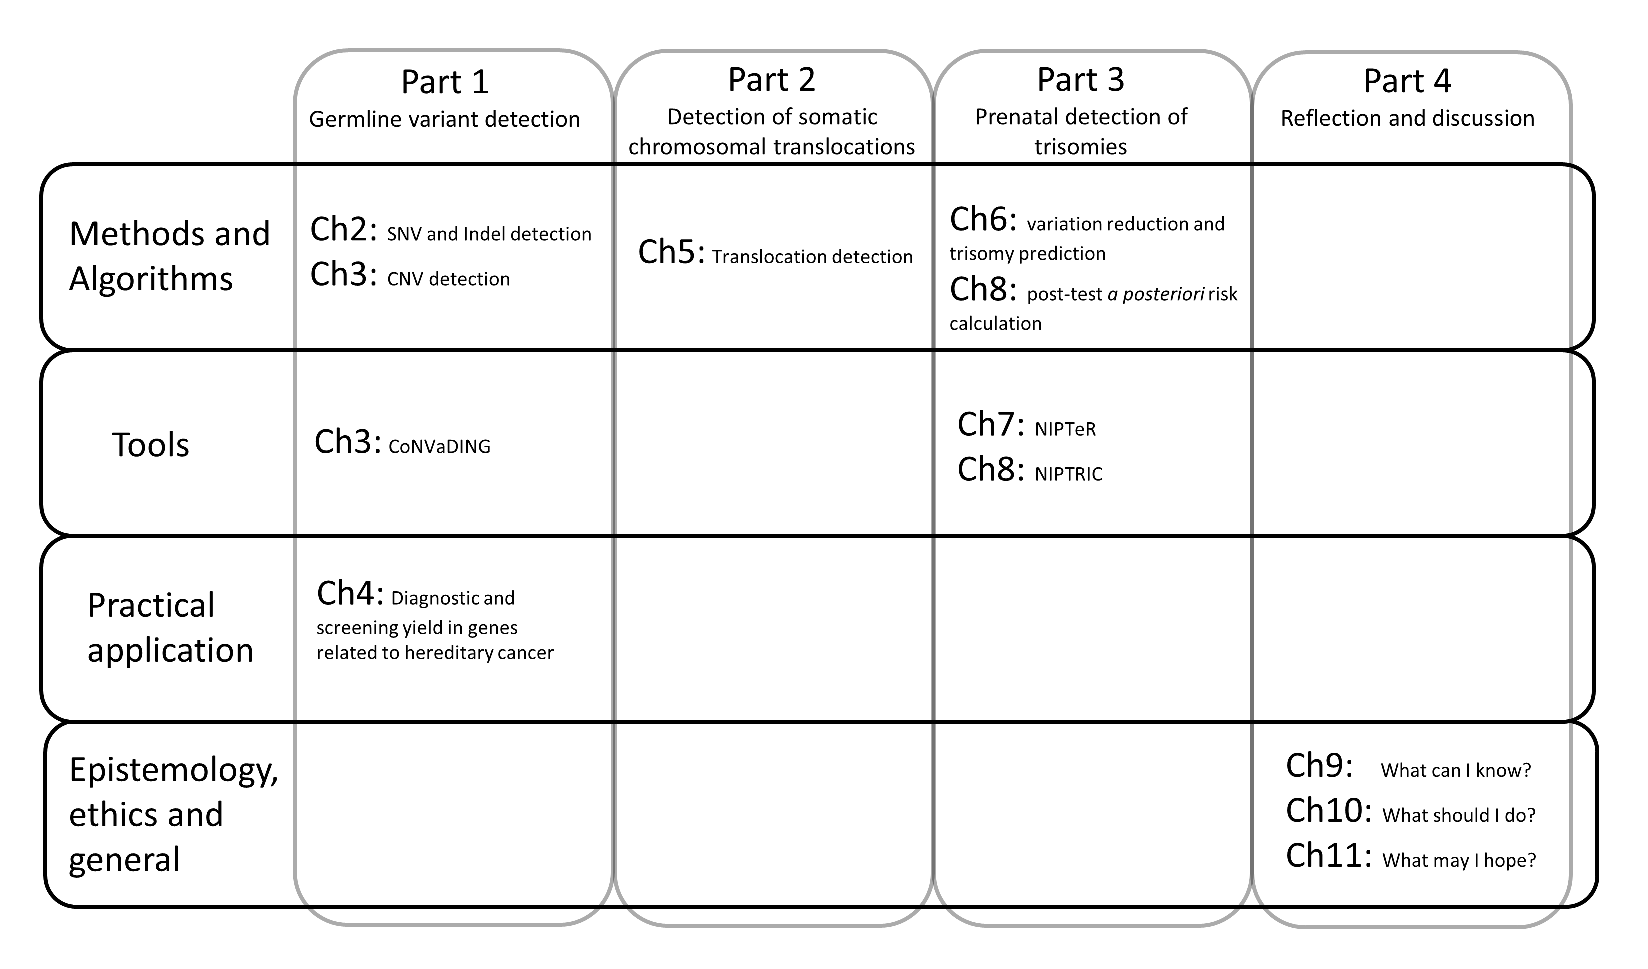
\includegraphics[width=1.0\linewidth]{img/Introduction_Fig3}
	\caption[Overview of the topics addressed in the thesis chapters ]{Overview of the topics addressed in the thesis chapters.}
	\label{fig:Introduction_Fig3}
\end{figure}

\subsection[Germline variant detection]{Part 1:  Germline variant detection \newline (chapters 2, 3 and 4)}\label{Part 1}
The most prevalent germline variants – SNVs, indels and small CNVs – were conventionally analyzed mainly using Sanger sequencing for SNV and indel detection and MLPA to detect CNVs. 
However, only a short stretch of DNA can be analyzed in each measurement using these techniques, limiting the number of genes that can by analyzed in a single experiment. 
In chapter 2 we set out to implement tNGS as a stand-alone diagnostic test to enable analysis of a large set of genes in a single test and replace Sanger sequencing in clinical diagnostics. For this we developed, validated and established quality criteria for a tNGS genepanel to detect SNVs and indels with high sensitivity and specificity in 48 genes involved in cardiomyopathies, ultimately demonstrating that tNGS is a technique suitable for diagnostic use. 
In chapter 3 we further expand the application of tNGS and enable simultaneous detection of CNVs up to the single exon level, next to SNVs and indels. 
Because it is likely in tNGS that CNV breakpoints are located outside targeted regions, CNVs can only be inferred through analysis of read depth. 
However, laboratory-induced variability of read depth is larger than biological variability. 
To look through the experimental noise and detect (single-exon) CNV in tNGS data, we introduce new algorithms with strict quality control that we implement in the open-source tool CoNVaDING (\textbf{\underline{Co}}py \textbf{\underline{N}}umber \textbf{\underline{Va}}riation \textbf{\underline{D}}etection \textbf{\underline{I}}n \textbf{\underline{N}}ext-generation sequencing \textbf{\underline{G}}ene panels). 
In chapter 4 we set out to use the tools and methods developed in the previous chapters in the context of hereditary cancer, for which we have analyzed 85 genes in 2,090 patients and 1,326 individuals from the general Dutch population. 
The first goal here was to determine the diagnostic yield, focusing on genes with a relation to the cancer type warranting referral. 
The second goal was to determine the findings if, in addition to these genes, we search for pathogenic or likely pathogenic variants in genes without such a relation (secondary findings), and how often variants leading to a cancer predisposition occur in the general Dutch population. 

\subsection[Detection of somatic chromosomal translocations]{Part 2: Detection of somatic chromosomal \newline translocations (chapter 5)}\label{Part2}
The second part of this thesis consists of a single chapter that focuses on somatic translocation detection. 
In current hematological malignancy diagnostics SVs, including translocations, are detected using various conventional techniques. 
Using karyotyping, large rearrangements are detected on a single-cell basis. 
However, this technique is unable to detect some so-called cryptic translocations. 
FISH and RT-PCR are needed to detect those, but these techniques can only target one SV or fusion-gene at a time. 
In chapter 5 we aim to develop an NGS-based technique to target 18 genes and detect translocations involving one of those genes commonly involved in acute leukemia, regardless of their translocation partner, to be suitable for use as a first-line screening tool in diagnostics. 
For this we make use of Targeted Locus Amplification (TLA) \cite{de_Vree_2014} to create a multiplex TLA acute leukemia gene panel. In addition to the genes themselves, our panel captures DNA physically close to the targeted genes, which enables the capture and detection of chromosomal translocation partners even if they are not in the targeted panel. 
We develop analysis and interpretation strategies and demonstrate for several targeted genes that the panel detects translocations involving those genes at 10\% aberrant cells. 
We conclude that multiplex TLA is a promising technique that it needs further optimization before it can replace conventional methods.

\subsection[Prenatal detection of trisomies]{Part 3: Prenatal detection of trisomies \newline (chapters 6, 7 and 8)}\label{Part3}
Part three of this thesis is dedicated to NIPT. Where conventional methods for prenatal trisomy detection, such as karyotyping, FISH, QF-PCR or array, rely on invasive procedures, NIPT can be performed using ultralow-coverage NGS data. Using a basic sample preparation with as few PCR cycles as possible, the short cfDNA fragments are made available for sequencing. 
Several algorithms are described in the literature to analyze such ultralow-coverage NGS data to predict the presence of a trisomy \cite{Chiu_2008,Fan_2010,Sehnert_2011}. 
These strategies rely on the comparison of the sample of interest to a group of non-trisomy control samples to determine if significantly more sequence reads are present that originate from DNA fragments of the potential trisomic chromosome. 
Because cffDNA is mixed with maternal DNA, a trisomy will only cause a small increase in the fraction of reads of the chromosome involved. 
Therefore it is important to make the variability in chromosomal fractions as small as possible between samples. 
In chapter 6 we introduce novel algorithms to analyze ultralow-coverage NGS data and obtain a higher sensitivity for trisomy detection than found using earlier described calculations. 
In addition, we create a quality metric that can be used to detect if the available reference samples are suitable for comparison with the sample analyzed. 
In chapter 7 we describe \textsl{NIPTeR}, an open-source R package that makes the algorithms developed in chapter 6 available along with the algorithms described in the literature for analysis of NIPT data. 

Two women receiving a similar test result from NIPT do not necessarily have a similar risk of carrying a child with a trisomy. 
In chapter 8 we focus on the clinical interpretation of the NIPT result, taking into account not only biological and technical characteristics of the test, but also the population to which the woman being tested belongs. 
Including these pre-test conditions in the interpretation might result in different risk profiles for women from different risk-groups who have the same raw test result. 
We created algorithms to calculate such a personalized post-test risk for a specific fetal trisomy and made these available in NIPTRIC, an online calculator. 

\subsection[Reflection and discussion]{Part 4: Reflection and discussion \newline (Chapters 9, 10 and 11)}\label{Part4}
Inspired by the three questions posed by Immanuel Kant in his \textsl{Kritik der reinen Vernunft} published in 1781/1787: “what can I know?”, “what should I do?” and “what may I hope?” \cite{Kant_1781a}[p.728], in part four of this thesis I reflect on and discuss the methods, tools and algorithms described in this thesis. 
In chapter 9 I look back on the chapters from an epistemological point of view. 
In genetic diagnostics we infer the genetic or genomic constitution of a person through a measurement outcome. 
I elaborate on the concept of noise that I define as ‘everything that, from a certain perspective, blocks the path between reality and measurement outcome’. 
Throughout this thesis we are battling four types of such noise: biological noise, laboratory-induced noise, sequencing noise and data analysis noise. 
The variants of interest are hidden behind this noise, but through innovative perspectives we are better able to look through the noise and correctly interpret measurement outcomes. 

In chapter 10 I make an ethical reflection on the technologies introduced in this thesis. I use the theories of Peter-Paul Verbeek who states that artefacts are morally charged and mediate human action \cite{Verbeek_2011}[p.21]. 
I try to uncover intended and unintended moral consequences of the availability of the methods, tools and algorithms presented in this thesis. 

In chapter 11 I address the last question of Kant: ‘what may I hope?’ and put the work presented in this thesis in broader perspective in the general discussion and give future perspectives on developments in NGS DNA analysis.

